% =============================================================================
% 3. PATHCAST ARCHITECTURE
% Target: 1.5 pages (~750 words)
% Source: cap4 §4.1 (sec:method-overview)
% Status: SKELETON — migrate Definition 4.1, Figure 4.1, design principles,
%         and consolidate the five stage contracts into a single table.
% =============================================================================

\section{PATHCAST Architecture}
\label{sec:architecture}

% ---------- §3.1 Pipeline definition ----------
\subsection{Pipeline Definition}
\label{sec:arch-pipeline}

PATHCAST is defined as a composition of four sequential transformation
stages and one parallel enhancement component:

\begin{definition}[PATHCAST Pipeline]
\label{def:pipeline}
The PATHCAST pipeline is the function composition
\begin{equation}
\label{eq:pipeline}
\mathcal{F} = \mathcal{S}_4 \circ \mathcal{S}_3 \circ \mathcal{S}_2 \circ \mathcal{S}_1
\end{equation}
where the stage signatures are
\begin{align}
\mathcal{S}_1 &: \mathcal{R} \to \mathcal{L}
    && \text{(Event Log Construction)} \label{eq:stage1-sig} \\
\mathcal{S}_2 &: \mathcal{L} \to (M, \Phi, S)
    && \text{(Process Mining)} \label{eq:stage2-sig} \\
\mathcal{S}_3 &: (\mathcal{L}, S) \to (P, N, B, \hat{F}, \pi)
    && \text{(Stochastic Modeling)} \label{eq:stage3-sig} \\
\mathcal{S}_4 &: (P, \hat{F}, s_0, M_{\text{sim}}) \to \hat{\mathcal{D}}
    && \text{(Monte Carlo Simulation)} \label{eq:stage4-sig}
\end{align}
together with a parallel enhancement component
\begin{equation}
\label{eq:ml-sig}
\mathcal{S}_{\text{ML}} : (\mathcal{L}, \Phi, P, N) \to (\hat{f}, \mathbf{w})
\quad \text{(ML Enhancement)}.
\end{equation}
\end{definition}

Notation: $\mathcal{R}$ denotes the input repositories;
$\mathcal{L}$ the structured event log; $M$ the discovered process
model; $\Phi$ the process metrics vector; $S = S_T \cup S_A$ the state
space; $P$ the Markov transition matrix; $N = (I-Q)^{-1}$ the
fundamental matrix; $B = NR$ the absorption probability matrix;
$\hat{F}$ the empirical sojourn-time distributions; $\pi$ the
stationary distribution; $\hat{\mathcal{D}}$ the empirical forecast
distribution; $\hat{f}$ the trained ML predictor; $\mathbf{w}$ the
feature-importance vector.

% ---------- §3.2 Architecture figure ----------
\subsection{Pipeline Architecture}
\label{sec:arch-figure}

Figure~\ref{fig:pipeline-architecture} illustrates the pipeline with
its data flows.

\begin{figure}[htbp]
\centering
\resizebox{0.95\linewidth}{!}{%
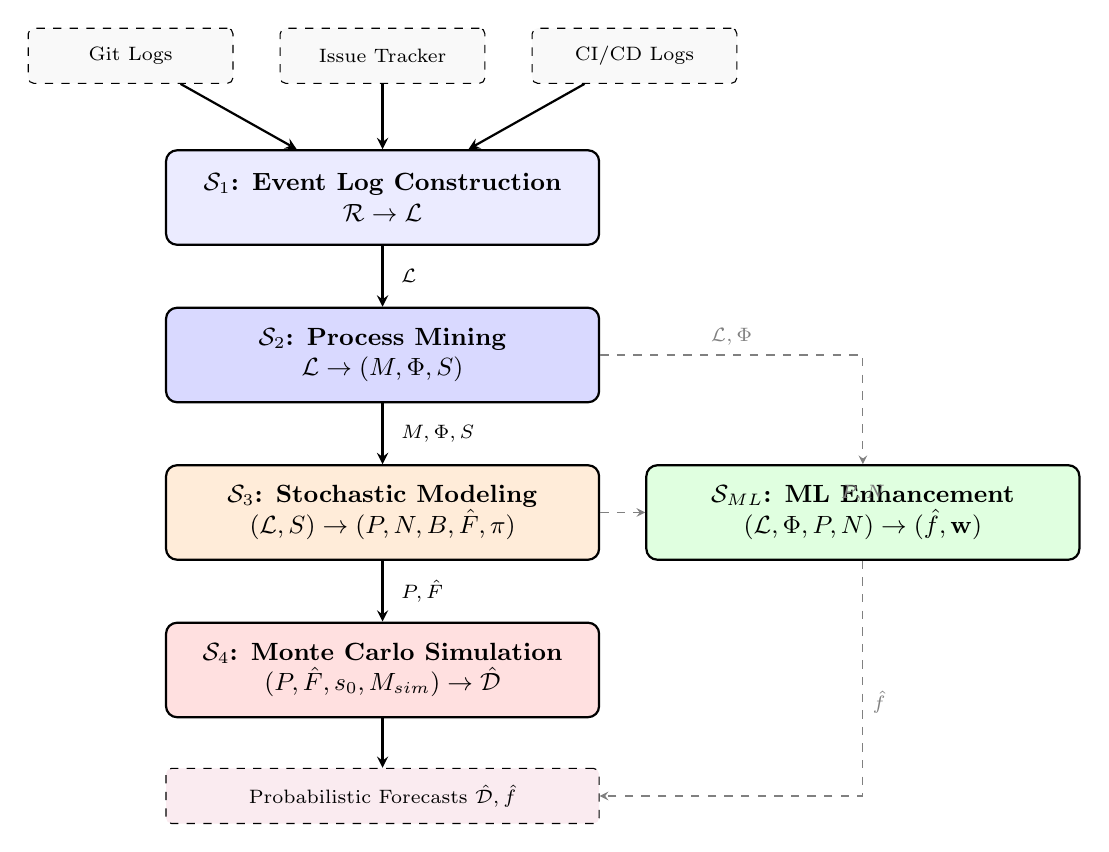
\begin{tikzpicture}[
    node distance=1.6cm,
    stage/.style={rectangle, draw, thick, rounded corners=4pt,
                  minimum width=5.5cm, minimum height=1.2cm,
                  align=center, font=\small},
    data/.style={rectangle, draw, dashed, rounded corners=2pt,
                 minimum width=2.6cm, minimum height=0.7cm,
                 align=center, font=\scriptsize, fill=gray!5},
    arrow/.style={->, thick, >=stealth},
    darrow/.style={->, dashed, >=stealth, gray},
    lbl/.style={font=\scriptsize, midway, right, xshift=3pt}
]
    \node[data] (git) at (-3.2, 0) {Git Logs};
    \node[data] (jira) at (0, 0) {Issue Tracker};
    \node[data] (ci) at (3.2, 0) {CI/CD Logs};

    \node[stage, fill=blue!8,  below of=jira, yshift=-0.2cm] (s1) {%
      \textbf{$\mathcal{S}_1$: Event Log Construction}\\
      $\mathcal{R} \to \mathcal{L}$};
    \node[stage, fill=blue!15, below of=s1,   yshift=-0.4cm] (s2) {%
      \textbf{$\mathcal{S}_2$: Process Mining}\\
      $\mathcal{L} \to (M, \Phi, S)$};
    \node[stage, fill=orange!15, below of=s2, yshift=-0.4cm] (s3) {%
      \textbf{$\mathcal{S}_3$: Stochastic Modeling}\\
      $(\mathcal{L}, S) \to (P, N, B, \hat{F}, \pi)$};
    \node[stage, fill=red!12,  below of=s3,   yshift=-0.4cm] (s4) {%
      \textbf{$\mathcal{S}_4$: Monte Carlo Simulation}\\
      $(P, \hat{F}, s_0, M_{\text{sim}}) \to \hat{\mathcal{D}}$};
    \node[stage, fill=green!12, right of=s3,  xshift=4.5cm] (ml) {%
      \textbf{$\mathcal{S}_{\text{ML}}$: ML Enhancement}\\
      $(\mathcal{L},\Phi,P,N) \to (\hat{f}, \mathbf{w})$};
    \node[data, below of=s4, yshift=-0.0cm, minimum width=5.5cm, fill=purple!8]
      (output) {Probabilistic Forecasts $\hat{\mathcal{D}}, \hat{f}$};

    \draw[arrow] (git) -- (s1);
    \draw[arrow] (jira) -- (s1);
    \draw[arrow] (ci) -- (s1);
    \draw[arrow] (s1) -- (s2) node[lbl] {$\mathcal{L}$};
    \draw[arrow] (s2) -- (s3) node[lbl] {$M,\Phi,S$};
    \draw[arrow] (s3) -- (s4) node[lbl] {$P,\hat{F}$};
    \draw[arrow] (s4) -- (output);

    \draw[darrow] (s2) -| (ml) node[font=\scriptsize, above, pos=0.25] {$\mathcal{L},\Phi$};
    \draw[darrow] (s3) -- (ml) node[font=\scriptsize, above] {$P,N$};
    \draw[darrow] (ml) |- (output) node[font=\scriptsize, right, pos=0.3] {$\hat{f}$};
\end{tikzpicture}}
\caption{PATHCAST pipeline architecture. Solid arrows: primary
sequential pipeline; dashed arrows: ML enhancement data flows.}
\label{fig:pipeline-architecture}
\end{figure}

% ---------- §3.3 Design principles ----------
\subsection{Design Principles}
\label{sec:arch-principles}

The architecture is governed by three principles.
\textbf{(P1) Empirical grounding} --- every model parameter is estimated
from observed data; no \emph{a priori} distribution is assumed unless
empirically validated.
\textbf{(P2) Stage composability} --- each stage exposes a formal
input/output contract (Table~\ref{tab:contracts}) so that stages may be
independently tested, replaced or extended.
\textbf{(P3) Distributional outputs} --- the pipeline produces
probability distributions, not point estimates; every forecast is the
empirical distribution of $M_{\text{sim}}$ simulated outcomes.

% ---------- §3.4 Inter-stage contracts (CONSOLIDATED TABLE) ----------
\subsection{Inter-Stage Contracts}
\label{sec:arch-contracts}

\begin{table}[ht]
\centering
\caption{Inter-stage contracts. Each stage is specified by its input,
output and key postconditions. Full specifications are given in
Section~\ref{sec:stages}.}
\label{tab:contracts}
\small
\begin{tabular}{@{}l l l p{5.5cm}@{}}
\toprule
\textbf{Stage} & \textbf{Input} & \textbf{Output} &
\textbf{Key Postconditions} \\
\midrule
$\mathcal{S}_1$    & $\mathcal{R}$
                   & $\mathcal{L}$
                   & Valid case ID, activity, timestamp per event;
                     timestamp-ordered within each trace. \\
$\mathcal{S}_2$    & $\mathcal{L}$
                   & $(M, \Phi, S)$
                   & $M$ sound; $\phi_{\text{fit}}, \phi_{\text{prec}}
                     \in [0,1]$; $|S_T|\ge1$, $|S_A|\ge1$. \\
$\mathcal{S}_3$    & $(\mathcal{L}, S)$
                   & $(P, N, B, \hat{F}, \pi)$
                   & $P$ row-stochastic; $(I-Q)$ invertible;
                     $\sum_j B_{ij}=1$. \\
$\mathcal{S}_4$    & $(P, \hat{F}, s_0, M_{\text{sim}})$
                   & $\hat{\mathcal{D}}$
                   & $|\hat{\mathcal{D}}| = M_{\text{sim}}$;
                     every trajectory absorbs or is flagged. \\
$\mathcal{S}_{\text{ML}}$ & $(\mathcal{L},\Phi,P,N)$
                   & $(\hat{f}, \mathbf{w})$
                   & Temporal hold-out enforced; AUC-ROC, F1, Brier
                     reported. \\
\bottomrule
\end{tabular}
\end{table}

The contracts establish the preconditions of the correctness theorem
proved in Section~\ref{sec:properties}
(Theorem~\ref{thm:pipeline-correctness}).
